\documentclass[conference, twoside]{IEEEtran}

\usepackage{tikz}
\newcommand{\onethird}{2.333333333cm}

\usetikzlibrary{positioning,fit,matrix}
\tikzstyle{architecture_node_nofill}=[rectangle, draw, minimum height=1cm,anchor=north west]
\tikzstyle{architecture_node_fullwidth}=[architecture_node_nofill,minimum width=7cm]
\tikzstyle{architecture_box}=[draw=black,dashed,anchor=north west]
\tikzstyle{architecture_no_fill}=[fill=none] % To disable all fills
\usetikzlibrary{calc}

\definecolor{lightred}{HTML}{EA2424}
\definecolor{red}{HTML}{D0021B}
\definecolor{lightblue}{HTML}{7D9FC7}
\definecolor{blue}{HTML}{4A90E2}
\definecolor{purple}{HTML}{7571A1}
\definecolor{green}{HTML}{70A500}
\definecolor{lightgreen}{HTML}{C1FF7D}
\definecolor{lightyellow}{HTML}{F8E71C}
\definecolor{yellow}{HTML}{F5A623}
\definecolor{lightorange}{HTML}{F56023}
\definecolor{orange}{HTML}{EB4400}
\definecolor{waterblue}{HTML}{6BE4C9}


\usepackage{cite}

% format citations
\renewcommand\citepunct{, }
\renewcommand\citeleft{[}
\renewcommand\citeright{]}
\renewcommand\citedash{--}


\begin{document}
    % TITLE & PUBLICATION ID

    \title{An effective approach to defect detection} %  on steel surfaces
    \IEEEpubid{0000--0000/00\$00.00 ̃\copyright ̃2019 IEEE }

    % AUTHORS

    \author{
        \IEEEauthorblockN{Antonio Terpin}
        \IEEEauthorblockA{Electronic Engineering, Scuola Superiore\\
        Università degli Studi di Udine\\
        Udine, Italia \\
        Email: terpin.antonio@spes.uniud.it}
        \and
        \IEEEauthorblockN{Claudio Verardo}
        \IEEEauthorblockA{Electronic Engineering, Scuola Superiore\\
        Università degli Studi di Udine\\
        Udine, Italia \\
        Email: verardo.claudio@spes.uniud.it}
    }

    \maketitle

    \begin{abstract}
    Quality control is a main issue in any industry. The need of assuring a human-like evaluation during products quality control has resulted in an active research aiming to develop an automatic defect detection scheme.
    In this paper an effective solution to defect detection on steel surfaces from images is presented. Firstly, a preprocessing step aiming to spot plausible defective areas is discussed. Lastly, the classification of these proposed regions is made. Hence, a proper segmentation scheme is described. Incidentally, a novel usage of the dilation factor in convolutional layers is introduced, providing an effective approach to classifying images of different sizes.
\end{abstract}

\begin{IEEEkeywords}
    Defect Detection, Computer Vision, Deep Learning, Wavelet.
\end{IEEEkeywords}
    \section{Introduction}
    \begin{frame}{Introduction}
        \begin{abstract}
            Quality control is a main issue in any industry, and the automation of quality control process has become a hot topic in research. In this paper an effective solution to defect detection on steel surfaces from images is presented.
        \end{abstract}
        \vskip 0.5cm
        \begin{description}
            \item<1->[1.] Case study
            \item<2->[2.] Wavelet
            \item<3->[3.] Computer vision
        \end{description}
    \end{frame}
    % \subsection{Wavelet Analysis}
    \framepic{graphics/wavelets/wavelet}{
        \framefill
        \textcolor{black}{Wavelet}
        \vskip 0.5cm
    }

    \begin{frame}{Multi Resolution Analysis}
        \centering
        \onslide <1-> {
            \begin{block}{Goal}
                Approximate vectors of $L^2\left(\mathbb{R}\right)$ with variable degrees of resolution.
            \end{block}
        }
        \only <2> {
            \includegraphics[width=.6\textwidth]{graphics/wavelets/mra}
        }
        \only <3> {
            \includegraphics[width=.6\textwidth]{graphics/wavelets/mra-1}
        }
        \only <4> {
            \includegraphics[width=.6\textwidth]{graphics/wavelets/mra-2}
        }
        \only <5> {
            \includegraphics[width=.6\textwidth]{graphics/wavelets/mra-3}
        }
    \end{frame}

    \begin{frame}{Multi Resolution Analysis}
        \begin{block}{Axioms}
            \begin{equation}
                \cdots \subset V_{-2} \subset V_{-1} \subset V_0 \subset V_1 \subset V_2 \subset \cdots
            \end{equation}
            \begin{equation}
                \overline{\bigcup\limits_{n \in \mathbb{Z}} V_n} = L^2\left(\mathbb{R}\right)
            \end{equation}
            \begin{equation}
                \bigcap\limits_{n \in \mathbb{Z}} V_n = \left\{0\right\}
            \end{equation}
            \begin{equation}
                V_{n+1} = \mathcal{S}V_n
            \end{equation}
            \begin{equation}
                V_0 = \langle \left\{\tau^i\phi, i \in \mathbb{Z}\right\} \rangle \quad \exists \phi \in L^2\left(\mathbb{R}\right)\rangle
            \end{equation}
        \end{block}
    \end{frame}

    \begin{frame}{Multi Resolution Analysis}
        \begin{block}{Scaling function}
            \begin{equation}
                V_1 \supset V_0, \phi \in V_1
            \end{equation}
            \begin{equation}
                \left\{\mathcal{S}\tau^i\phi = \tau^{i/2}\mathcal{S}\phi, i \in \mathbb{Z}\right\} \; \text{orthonormal basis of } V_1
            \end{equation}
            \begin{equation}
                    \phi = \sum_{i \in \mathbb{Z}} g_i \tau^{i/2} \mathcal{S} \phi
            \end{equation}
        \end{block}
    \end{frame}

    \begin{frame}{Multi Resolution Analysis}
        \begin{block}{Wavelet}
            \begin{equation}
                V_{n+1} \supset V_n \Rightarrow \exists W_n \colon V_{n+1} = V_n \oplus W_n
            \end{equation}
            \begin{equation}
                \left\{\tau^i\psi\right\}_{i \in \mathbb{Z}} = W_0
            \end{equation}
            \begin{equation}
                \psi = \sum_{i \in \mathbb{Z}} h_i \tau^{i/2}\mathcal{S}\phi\quad\psi \in V_1
            \end{equation}
            \begin{equation}
                \langle \psi, \tau^i \psi \rangle = \delta_i
            \end{equation}
            \begin{equation}
                \langle \tau^j\psi, \tau^i \phi \rangle = 0
            \end{equation}
        \end{block}
    \end{frame}

    \begin{frame}
        \frametitle{Multi Resolution Analysis}
        \framesubtitle{Filter banks}
        \centering 
        \begin{tikzpicture}
            % High res
            \node[anchor= west] (highres) at (0,0) {$V_{n+1}$};
            % Low res
            \node[rectangle, draw, anchor= west, minimum height=0.75cm, minimum width=1.5cm] (g) at (3,2) {g};
            \node[circle, draw, anchor= west] (downsampleg) at (6,2) {$\downarrow 2$};
            \node[anchor= west] (lowres) at (8,2) {$V_n$};
            % Details
            \node[rectangle, draw, anchor= west, minimum height=0.75cm, minimum width=1.5cm] (h) at (3,-2) {h};
            \node[circle, draw, anchor= west] (downsampleh) at (6,-2) {$\downarrow 2$};
            \node[anchor= west] (details) at (8,-2) {$W_n$};

            \draw[->] (1,0) -- (2,0) -- (2,2) -- (3,2);
            \draw[->] (1,0) -- (2,0) -- (2,-2) -- (3,-2);

            \draw[->] (4.5,2) -- (6,2);
            \draw[->] (4.5,-2) -- (6,-2);

            \draw[->] (7,2) -- (8,2);
            \draw[->] (7,-2) -- (8,-2);

        \end{tikzpicture}
    \end{frame}

    \begin{frame}
        \frametitle{Wavelet: Example application}
        \framesubtitle{Detect abrupt changes}

        \centering
        \vskip -1cm
        $$s_1(t) = 2\sin\left(2\pi 10f_0 t\right) + \sin\left(2\pi 50f_0 t\right) + 10\delta\left(t - \frac{1}{2f_0}\right)$$
        \only<1> {
            \includegraphics[height=0.6\textheight]{graphics/wavelets/signal1}
        }
        \only<2> {
            \begin{columns}[onlytextwidth]
                \column{0.5\textwidth}
                \includegraphics[width=\textwidth]{graphics/wavelets/detect-abrupt-changes-fft}
                \column{0.5\textwidth}
                \includegraphics[width=\textwidth]{graphics/wavelets/detect-abrupt-changes-cwt}
            \end{columns}
        }

    \end{frame}

    \begin{frame}
        \frametitle{Wavelet: Example application}
        \framesubtitle{Detect temporal trends}
        $$f_{s_2} = e^t;\quad s_2 = \sin\left(2*pi*f_{s_2}t\right)$$
        \begin{columns}[onlytextwidth]
            \column{0.5\textwidth}
            \only<1-2> {
                \includegraphics[width=\textwidth]{graphics/wavelets/frequency-signal-2}
            }
            \only<3-4> {
                \includegraphics[width=\textwidth]{graphics/wavelets/detect-pattern-fft}
            }
            \column{0.5\textwidth}
            \only<2> {
                \includegraphics[width=\textwidth]{graphics/wavelets/signal2}
            }
            \only<4> {
                \includegraphics[width=\textwidth]{graphics/wavelets/detect-pattern-cwt}
            }
        \end{columns}
        
    \end{frame}


    \subsection{Computer Vision}
    \framepic{graphics/computervision/computer-vision}{
        \framefill
        \textcolor{white}{Computer Vision}
        \vskip 0.5cm
    }
    \begin{frame}{Computer Vision}
        \begin{block}{Classification Task}
            To determine to which of a set of \textbf{categories} a given object belongs to.
        \end{block}
        \begin{columns}[onlytextwidth]
            \column{0.3\textwidth}
            \centering
            \includegraphics[width=\textwidth]{graphics/computervision/classification-image.jpeg}
            \onslide <2-> {
                \column{0.4\textwidth}
                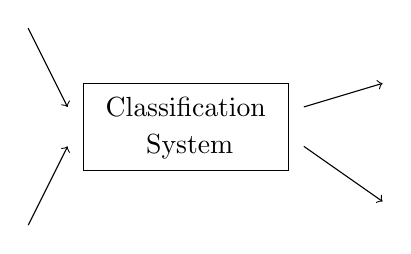
\begin{tikzpicture}
                    \node at (0,0) {Classification};
                    \node at (0.05,-0.5) {System};
                    \node[rectangle, draw, minimum width=2.6cm, minimum height=1.1cm, anchor=north west] at (-1.3,0.3) {};
                    \draw[->] (-2,1) -- (-1.5,0);
                    \draw[->] (-2,-1.5) -- (-1.5,-0.5);
                    \onslide <3-> {
                        \draw[->] (1.5,0) -- (2.5,0.3);
                        \draw[->] (1.5,-0.5) -- (2.5,-1.2);
                    }
                \end{tikzpicture}
            }
            \onslide <3-> {
                \column{0.2\textwidth}
                \vskip -0.5cm Output \vskip 0.5cm
                \begin{columns}[onlytextwidth]
                    \column{0.5\textwidth}
                        \begin{tabular}{|c|}
                            \hline
                            $0.03$\\\hline
                            \cellcolor{UniBlue}\textcolor{white}{$0.77$}\\\hline
                            $\vdots$\\\hline
                            $0.12$\\\hline
                        \end{tabular}
                    \column{0.5\textwidth}
                        \vskip -0.2cm
                        \begin{tabular}{c}
                            \\
                            \textcolor{UniBlue}{Child}\\
                            \\
                            \\
                        \end{tabular}
                \end{columns}
            }
        \end{columns}
    \end{frame}

    \begin{frame}{Computer Vision}
        \begin{block}{Object Localization Task}
            To find a given number (usually one) of items in a given context, predicting both their position and their class. \\
            \textbf{Remark.} Position is usually given as a bounding box.
        \end{block}
        \begin{columns}[onlytextwidth]
            \column{0.45\textwidth}
            \onslide <2-> {
                \includegraphics[width=\textwidth]{graphics/computervision/localization-input}
            }
            \column{0.45\textwidth}
            \onslide <3-> {
                \includegraphics[width=\textwidth]{graphics/computervision/localization-output}
            }
        \end{columns}
    \end{frame}

    \begin{frame}{Computer Vision}
        \onslide<1-> {
            \begin{block}{Object Detection Task}
                To \textbf{localize} any number of items in a given context, allowing either zero or any finite number of objects.
            \end{block}
        }
        \onslide<2-> {
            \begin{alertblock}{Remark.}
                The constraint on the number of object is \emph{a priori}. Indeed, a localization system will always look for a fixed number of objects, whereas a detection system is trained to be able to spot a variable number of objects in each input.
            \end{alertblock}
        }
    \end{frame}

    \begin{frame}{Computer Vision}
        \onslide <1-> {
            \begin{block}{Image Segmentation}
                Pixel-wide classification of the image. \textbf{Remark.} Image segmentation can be consider either the preemptive step to classification or the output of a classification system.
            \end{block}
        }
        \onslide <2-> {
            \vskip -0.5cm 
            \begin{exampleblock}{Example: Pixel-based image segmentation.}
                This family considers some distance defined over the image domain to segmentate it.
            \end{exampleblock}
        }
        \onslide <3-> {
            \vskip -0.5cm 
            \begin{exampleblock}{Example: Edge-based image segmentation.}
                This family uses an edge-detector algorithm, along with denoising and thresholding considerations, to solve the boundary detection problem.
            \end{exampleblock}
        }
    \end{frame}

    % \begin{frame}
    %     \frametitle{Pixel-based image segmentation}
    %     \framesubtitle{Whatershed}
    %     \begin{columns}[onlytextwidth]
    %         \column{0.5\textwidth}
    %         \includegraphics[width=\textwidth]{graphics/computervision/whatershed-plane}
    %         \column{0.5\textwidth}
    %         \includegraphics[width=\textwidth]{graphics/computervision/whatershed-surf}
    %     \end{columns}
    %     \only <1> {
    %         \begin{block}{Whatershed and immersion}
    %             The above pictures both show the same function defined over a 2D domain. Suppose to immerse the above right surface in some liquid, which gradually fill the two holes.
    %         \end{block}
    %     }
    %     \only <2> {
    %         \begin{block}{Whatershed and immersion}
    %             At some point the two volumes of liquid will meet, in particular they will flood at the same time over the green colored surface region.
    %         \end{block}
    %     }
    %     \only <3> {
    %         \begin{block}{Whatershed and immersion}
    %             This region is called whatershed and differentiates two areas of the image. Hence, an image can be segmentated considering its whatersheds.
    %         \end{block}
    %     }
    % \end{frame}

    % \begin{frame}
    %     \frametitle{Pixel-based image segmentation}
    %     \framesubtitle{Whatershed}
    %     % \includegraphics[width=\textwidth]{graphics/whatershed-plane}
    %     TODO insert example image\\
    %     % \includegraphics[width=\textwidth]{graphics/whatershed-surf}
    %     TODO insert example image
    % \end{frame}

    % \begin{frame}
    %     \frametitle{Pixel-based image segmentation}
    %     \framesubtitle{Whatershed}
    %     Let $\mathcal{D} \subset \mathbb{R}_+^2$ be a $2D$ domain, and $\mathcal{I} \colon \mathcal{D} \rightarrow \mathbb{R}_+$. Denote $\displaystyle h_m \triangleq \min_{\underline{x} \in \mathcal{D}}\mathcal{I}(\underline{x})$, $\displaystyle h_M \triangleq \max_{\underline{x} \in \mathcal{D}}\mathcal{I}(\underline{x})$, $T_h\left(\mathcal{I}\right) \triangleq \left\{\underline{p} \in \mathcal{D}, \mathcal{I}(\underline{p}) \leq h\right\}$.
    % \end{frame}

    % \begin{frame}
    %     \frametitle{Pixel-based image segmentation}
    %     \framesubtitle{Whatershed}
    %         \begin{itemize}
    %             \item Def, th, alg
    %             \item Example results
    %         \end{itemize}
    % \end{frame}
    \subsection{Deep Learning}
    \framepic{graphics/deeplearning/deep-learning}{
        \framefill
        \textcolor{white}{Deep Learning}
        \vskip 0.5cm
    }

    \begin{frame}{Computer Vision}
        \begin{block}{Classification Task}
            To determine to which of a set of \textbf{categories} a given object belongs to.
        \end{block}
        \begin{columns}[onlytextwidth]
            \column{0.3\textwidth}
            \centering
            \includegraphics[width=\textwidth]{graphics/computervision/classification-image.jpeg}
            \onslide <2-> {
                \column{0.4\textwidth}
                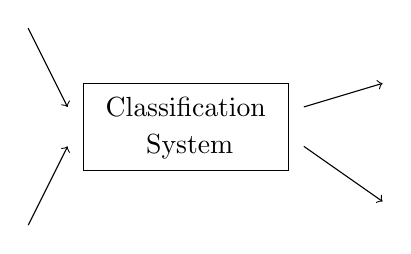
\begin{tikzpicture}
                    \node at (0,0) {Classification};
                    \node at (0.05,-0.5) {System};
                    \node[rectangle, draw, minimum width=2.6cm, minimum height=1.1cm, anchor=north west] at (-1.3,0.3) {};
                    \draw[->] (-2,1) -- (-1.5,0);
                    \draw[->] (-2,-1.5) -- (-1.5,-0.5);
                    \onslide <3-> {
                        \draw[->] (1.5,0) -- (2.5,0.3);
                        \draw[->] (1.5,-0.5) -- (2.5,-1.2);
                    }
                \end{tikzpicture}
            }
            \onslide <3-> {
                \column{0.2\textwidth}
                \vskip -0.5cm Output \vskip 0.5cm
                \begin{columns}[onlytextwidth]
                    \column{0.5\textwidth}
                        \begin{tabular}{|c|}
                            \hline
                            $0.03$\\\hline
                            \cellcolor{UniBlue}\textcolor{white}{$0.77$}\\\hline
                            $\vdots$\\\hline
                            $0.12$\\\hline
                        \end{tabular}
                    \column{0.5\textwidth}
                        \vskip -0.2cm
                        \begin{tabular}{c}
                            \\
                            \textcolor{UniBlue}{Child}\\
                            \\
                            \\
                        \end{tabular}
                \end{columns}
            }
        \end{columns}
    \end{frame}

    \begin{frame}{Computer Vision}
        \begin{block}{Object Localization Task}
            To find a given number (usually one) of items in a given context, predicting both their position and their class. \\
            \textbf{Remark.} Position is usually given as a bounding box.
        \end{block}
        \begin{columns}[onlytextwidth]
            \column{0.45\textwidth}
            \onslide <2-> {
                \includegraphics[width=\textwidth]{graphics/computervision/localization-input}
            }
            \column{0.45\textwidth}
            \onslide <3-> {
                \includegraphics[width=\textwidth]{graphics/computervision/localization-output}
            }
        \end{columns}
    \end{frame}

    \begin{frame}{Computer Vision}
        \onslide<1-> {
            \begin{block}{Object Detection Task}
                To \textbf{localize} any number of items in a given context, allowing either zero or any finite number of objects.
            \end{block}
        }
        \onslide<2-> {
            \begin{alertblock}{Remark.}
                The constraint on the number of object is \emph{a priori}. Indeed, a localization system will always look for a fixed number of objects, whereas a detection system is trained to be able to spot a variable number of objects in each input.
            \end{alertblock}
        }
    \end{frame}

    \begin{frame}{Computer Vision}
        \onslide <1-> {
            \begin{block}{Image Segmentation}
                Pixel-wide classification of the image. \textbf{Remark.} Image segmentation can be consider either the preemptive step to classification or the output of a classification system.
            \end{block}
        }
        \onslide <2-> {
            \vskip -0.5cm 
            \begin{exampleblock}{Example: Pixel-based image segmentation.}
                This family considers some distance defined over the image domain to segmentate it.
            \end{exampleblock}
        }
        \onslide <3-> {
            \vskip -0.5cm 
            \begin{exampleblock}{Example: Edge-based image segmentation.}
                This family uses an edge-detector algorithm, along with denoising and thresholding considerations, to solve the boundary detection problem.
            \end{exampleblock}
        }
    \end{frame}

    \begin{frame}{Training}
        \begin{block}{Forward propagation}
            The \emph{feedforward} neural network accepts an input $\underline{\underline{X}}$ and produce an output $\underline{y}$. The information from $\underline{\underline{X}}$ flows through the hidden units to produce $\underline{y}$. This is called \textbf{forward propagation}.
        \end{block}

        \begin{block}{Backward propagation}
            During the training the forward propagation can continue onward to evaluate a scalar cost $J\left(\underline{\underline{\theta}}\right)$. The \textbf{back-propagation} algorithm is a numerically efficient way to compute cost gradient, in order to perform gradient descent.
        \end{block}    
    \end{frame}

    \begin{frame}{Deep Learning}
        \includegraphics[width=\textwidth]{graphics/deeplearning/nn}
    \end{frame}

    \begin{frame}
        \frametitle{Training}
        \framesubtitle{Backpropagation (proof)}
        \centering
        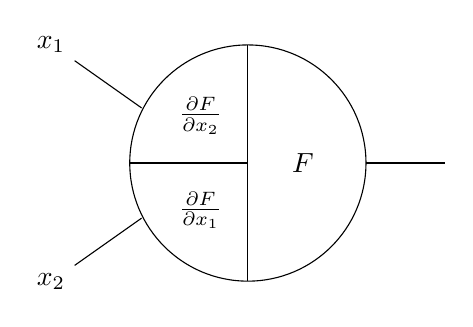
\begin{tikzpicture}
            \node[circle, draw, minimum width=3cm, minimum height=3cm] at (0,0) {};
            \node at (0.7,0) {$F$};
            \node at (-0.6,-0.6) {$\frac{\partial F}{\partial x_1}$};
            \node at (-0.6,0.6) {$\frac{\partial F}{\partial x_2}$};
            \node at (-2.5,1.5) {$x_1$};
            \node at (-2.5,-1.5) {$x_2$};

            \draw (0,0) -- (-1.5,0);
            \draw (0,-1.5) -- (0,1.5);
            \draw (1.5, 0) -- (2.5,0);

            \draw (-1.35, 0.7) -- (-2.2,1.3);
            \draw (-1.35, -0.7) -- (-2.2,-1.3);
        \end{tikzpicture}

        \vskip 0.5cm
        
        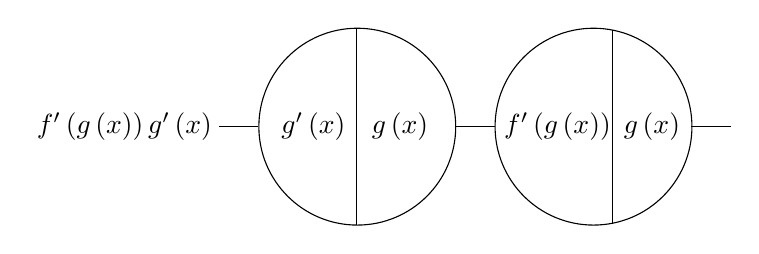
\begin{tikzpicture}
            \node at (-.7,0) {$f'\left(g\left(x\right)\right)g'\left(x\right)$};

            \draw (0.5,0) -- (1,0);

            \node[circle, draw, minimum width=2.5cm, minimum height=2.5cm, anchor=west] at (1,0) {};
            \node at (1.7, 0) {$g'\left(x\right)$};
            \node at (2.8, 0) {$g\left(x\right)$};
            \draw (2.25, 1.25) -- (2.25, -1.25);

            \draw (3.5, 0) -- (4, 0);

            \node[circle, draw, minimum width=2.5cm, minimum height=2.5cm, anchor=west] at (4,0) {};
            \node at (4.8, 0) {$f'\left(g\left(x\right)\right)$};
            \node at (6, 0) {$g\left(x\right)$};
            \draw (5.5, 1.23) -- (5.5, -1.23);

            \draw (6.5, 0) -- (7, 0);

        \end{tikzpicture}
    \end{frame}

    \begin{frame}{Convolutional Networks}
        \includegraphics[width=\textwidth]{graphics/deeplearning/cnn}
        \vskip 0.5cm
        \begin{exampleblock}{Motivation}
            \begin{enumerate}
                \item Sparse interactions
                \item Parameter sharing
                \item Equivariant representations
                \item Biologically inspired artificial intelligence
            \end{enumerate}
        \end{exampleblock}
    \end{frame}

    \begin{frame}{Convolutional Networks}
        \includegraphics[width=\textwidth]{graphics/deeplearning/cnn}
        \onslide <1-> {
            \begin{block}{Convolutional neural networks (CNN)}
                CNNs are a specialized kind of neural network for processing data that has a known grid-like topology.
            \end{block}
        }
        \onslide <2-> {
            \begin{block}{Convolutional neural networks (CNN) - 2}
                CNNs are neural networks that use convolution in place of general matrix multiplication in at least one of their layers.
            \end{block}
        }
    \end{frame}


    \section{Architecture overview}\label{section:architecture}
    \begin{figure}
        \centering
        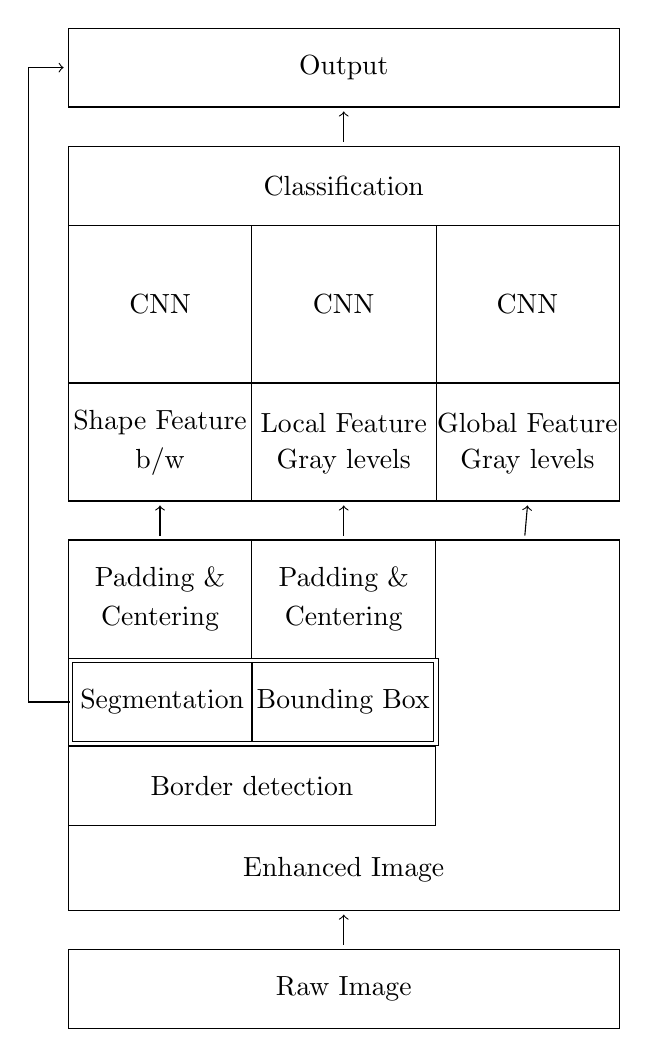
\begin{tikzpicture}

            % \draw[help lines] (0,0) grid (8.5,16);

            % Output
            \node[architecture_node_fullwidth,fill=waterblue,architecture_no_fill] (output) at (1,16) {Output};

            % Classificator
            % \node[architecture_box,minimum width=7.2cm,minimum height=4.7cm] (classification_architecture) at (.9,14.6) {};
            \node[architecture_node_fullwidth,fill=purple,architecture_no_fill] (classification) at (1,14.5) {Classification};
                    % CNN
                \matrix[architecture_node_nofill,minimum width=\onethird,minimum height=2cm,inner sep=0mm,fill=blue,architecture_no_fill] (cnn) at (1,13.5) {
                    \node {CNN}; & \node (cnn_local) {CNN}; & \node {CNN}; \\
                };
                \draw[black] (cnn_local.north east)--(cnn_local.south east);
                \draw[black] (cnn_local.north west)--(cnn_local.south west);

                    % INPUT
                \matrix[architecture_node_nofill,minimum width=\onethird,minimum height=1cm,inner sep=0mm,row sep=-0.51cm,fill=lightblue,architecture_no_fill] (cnn_features) at (1,11.5) {
                    \node (cnn_shape_feature) {Shape Feature}; & \node (cnn_local_feature) {Local Feature}; & \node (cnn_global_feature) {Global Feature}; \\
                    \node (cnn_shape_feature_color) {b/w}; & \node (cnn_local_feature_color) {Gray levels}; & \node (cnn_global_feature_color) {Gray levels}; \\
                };
                \draw[black] (cnn_local_feature.north east)--(cnn_local_feature_color.south east);
                \draw[black] (cnn_local_feature.north west)--(cnn_local_feature_color.south west);
            
            \draw[->] ($(classification.north) + (0,.05)$) -- ($(output.south) + (0,-0.05)$);

            % INPUT PREPROCESSING
                % Enhanced image
                \node[architecture_node_fullwidth,minimum height=4.7cm,fill=lightyellow,architecture_no_fill] (enhanced_image_box) at (1,9.5) {};
                \node[architecture_node_fullwidth,minimum height=1cm,anchor=south west,draw=none] (enhanced_image_label) at (1,4.8) {Enhanced Image};
                % \node[architecture_box,minimum width=7.2cm,minimum height=4.9cm] (preprocessing_architecture) at (.9,9.6) {};

                % Padding
                \matrix[architecture_node_nofill,minimum width=\onethird,minimum height=1cm,inner sep=0mm,row sep=-0.51cm,fill=lightred,architecture_no_fill] (cnn) at (1,9.5) {
                    \node (padding1) {Padding \&}; & \node (padding2) {Padding \&};\\
                    \node {Centering}; & \node (centering2) {Centering};\\
                };
                \draw[black] (padding2.north west)--(centering2.south west);

                % Segmentation & Bounding box
                \matrix[architecture_node_nofill,minimum width=\onethird - .6mm,minimum height=1cm,inner sep=.5mm,nodes={draw=black},fill=lightorange,architecture_no_fill,nodes={fill=orange,architecture_no_fill}] (segmentation_bounding_box) at (1,8) {
                    \node {Segmentation}; & \node {Bounding Box};\\
                };

                % Border detection & Region proposals
                \node[architecture_node_nofill,minimum width=2*\onethird,minimum height=1cm,fill=yellow,architecture_no_fill] (border) at (1,6.88) {Border detection};
            
            \draw[->] ($(segmentation_bounding_box.west) + (0.03,0)$) -- ($(segmentation_bounding_box.west) + (-0.5,0)$) -- ($(output.west) + (-0.5,0)$) -- ($(output.west) + (-0.05,0)$);
            \draw[->] ($(padding1.north) + (0,.05)$) -- ($(cnn_shape_feature_color.south) + (0,-0.05)$);
            \draw[->] ($(padding2.north) + (0,.05)$) -- ($(cnn_local_feature_color.south) + (0,-0.05)$);
            \draw[->] ($(enhanced_image_box.north) + (2.3cm,.05)$) -- ($(cnn_global_feature_color.south) + (0,-0.05)$);

            % Raw image
            \node[architecture_node_fullwidth,fill=green,architecture_no_fill] (rawim) at (1,4.3) {Raw Image};
            \draw[->] ($(rawim.north) + (0,.05)$) -- ($(enhanced_image_box.south) + (0,-0.05)$);

        \end{tikzpicture}
        \caption{Proposed defect detection system architecture}\label{fig:architecture}
    \end{figure}

    \par{
        The defect detection system architecture proposed in this paper is described in \emph{Figure \ref{fig:architecture}}.
    }

    \par{
        Steel surfaces pictures of $1600\times 256$ pixels are taken at the input of the process. Since they may be taken under different light exposure conditions, some preprocessing is made to enhance the quality of the image, e.g. histogram equalization or linear scaling. Moreover, the images considered have three equal colours levels, therefore they are converted into gray levels, to save space. This first step is further described in \emph{Section \ref{section:image_preprocessing}}.
    }
    \par{
        The aim of the architecture proposed in this paper is both to detect pixels representing steel imperfections and to classify those regions. Therefore, image segmentation is either obtained as an output of the system or it is needed in some step during the process. The latter situation can be achieved through a brute-force multi-scale sliding window, but to improve performances without reducing accuracy a particular implementation of a Region based CNN (R-CNN) \cite{ieee:7410526,ieee:7532516} is proposed in \emph{Section \ref{section:mc-cnn}}. This R-CNN uses a MC-CNN to combine and to consider separately interesting regions, which are called proposals and which are described in \emph{Section \ref{section:region_proposals}}.
    }
    \par{
        This reduces the computational cost of the system, compared with a naive sliding window.
    }
    \par{
        Moreover, both local and global information are combined to improve classification accuracy. This approach avoids the complexity of combining different scale information and handling windows with different classes of defects. A further description of this approach is provided in \emph{Section \ref{section:mc-cnn}}, whereas in \emph{Section \ref{section:further-work}} a challenger architecture is described, to compare the results of the proposed system with.
    }
    \par{
        One column of the MC-CNN is concerned with global information, and it is fed with the full enchanced image. Conceptually, this CNN learns to evaluate the probability of presence of the different types of defects in the whole surface picture. The other two columns consider local information instead. This local information is obtained from a further processing step, described in \emph{Section \ref{section:region_proposals}}. First, a contour detection algorithm (\emph{Section \ref{subsection:contour_detection}}) is used to spot proposals. Second, image segmentation (\emph{Section \ref{subsection:segmentation}}) is done, to feed the MC-CNN only with some interesting regions. This segmentation results in a black and white (b/w) map describing the shape of the plausible defects. One column of the MC-CNN is fed with this map, therefore it learns to classify regions only observing their border. The other column is fed with the portion of original image enveloped in the bounding box (\emph{Section \ref{subsection:bounding_box}}) of the map, hence, it is trained to consider luminance levels inside, outside and on the border of the considered proposals.
    }
    \par{
        Since defects may have different dimensions, the local information are centered in a $1600\times 256$ pixels black image.
    }
    \par{
        All the MC-CNN columns end with a softmax layer. However, they have different output size, as described in \emph{Section \ref{section:mc-cnn}}. Their results are then combined in order to properly classify the local regions.
    }
    \par{
        Finally, if the classification outcome labels the region as defective, segmentation coordinates are kept. When all the proposals of the considered image are processed, defective pixels of the same class are encoded together with RLE algorithm. If the surface is flawless, all this encodings are empty.
    }
    \section{Image preprocessing}\label{section:image_preprocessing}
    \par{
        In this section image preprocessing is introduced, and the raw image is enhanced to improve learning quality. In \ref{section:results} the contribution of preprocessing is evaluated.
    }
    \par{
        Firstly, since given images have three equal colours levels, they can be considered gray-levels. Therefore it is possible to shrink the space occupied on disk by discarding hue and saturation information and using only luminance.
    }
    \par{
        Rec.ITU-R BT.601-7 calculates luminance $\left(E\left[y\right]\right)$ as:
        $$ E\left[y\right] = 0.299 * R + 0.587 * G + 0.114 * B $$
        where $R,G,B$ are the three image channels. Observe that since $R = G = B$, also $E\left[y\right] = R = G = B$, which justifies the assumption that discarding hue and saturation does not affect effectiveness of the system, whereas improving space and computational efficiency. Luminance is denoted by $E\left[y\right]$ since brightness is named $y$ in literature, therefore the luminance, i.e. the physical intensity expected, is labeled in this way.
    }
    \par{
        Secondly, since pictures may be taken under different light exposure conditions, and since learning has heuristically be proven to be more effective if input assumptions are always the same, the luminance histogram of the image is normalized.
    }
    \par{
        Linear scaling ensure that all images gray levels spread over all the range of possible values. $\mathcal{I}\left(x,y\right)$ refers to the luminance level of pixel $\left(x,y\right)$ of image $\mathcal{I}$. Therefore, denoting with $G_{max}$ the greater luminance level (tipically $2^k - 1$ for some $k$), the luminance scaled image is obtained as:
        $$\mathcal{I}_{new}\left(x,y\right) = G_{max} \frac{\mathcal{I}\left(x,y\right) - \mathcal{I}_{min}}{\mathcal{I}_{max} - \mathcal{I}_{min}}$$
        $$\mathcal{I}_{max} = \max_{x,y} \mathcal{I}\left(x,y\right)\;;\quad\mathcal{I}_{min} = \min_{x,y} \mathcal{I}\left(x,y\right)$$
    }
    \par{
        However, histogram equalization is preferred over linear scaling.
    }
    \par{
        Indeed, although both linear scaling and histogram equalization are effective in spreading over all the spectrum the luminance levels of an image, the former only ensure that all the intensities are used whereas the latter is also concerned about the shape of the resulting histogram, which ideally should be flat.
    }
    \par{
        In fact, histogram equalization aims to transform a scalar image $\mathcal{I}$ such that all grey levels appear equally often in the transformed image $\mathcal{I}_{new}$, i.e.:
        \begin{equation*}
            H_{\mathcal{I}_{new}}(u) = \text{const} = \frac{N_{cols}N_{rows}}{G_{max} + 1} \quad 0 \leq u \leq G_{max}
        \end{equation*}
        Where $N_{cols}$ and $N_{rows}$ are, respectively, the number of columns and rows of the image. $H_{\mathcal{I}}(u)$ is the absolute frequency of luminance level $u$.
    }
    \par{
        However, this is not practically feasible, since identical value in $\mathcal{I}$ must be mapped on the same value of $\mathcal{I}$. Therefore, the transform is just an approximate solution.
    }
    \par{
        Intensities $u$ in $\mathcal{I}$ are mapped onto new intensities $v = g(u)$ by the gradation function $g$: 
        \begin{equation*}
            g(u) = c_{\mathcal{I}}(u) \cdot G_{max}
        \end{equation*}
        Where $c_{\mathcal{I}}$ is the relative cumulative frequency function.
    }
    \begin{figure}
        \includegraphics[width=\linewidth]{graphics/preprocessing/histeq-before}
        \includegraphics[width=\linewidth]{graphics/preprocessing/histeq-after}
        \caption{Hystogram of luminance distribution on sample image before and after equalization.}\label{fig:equalization}
    \end{figure}
    \par{
        In figure \ref{fig:equalization} the effects of equalization a sample image hystogram of luminance distribution are shown.
    }
    \begin{figure}
        \includegraphics[width=\linewidth]{graphics/preprocessing/histeq-before-image}
        \includegraphics[width=\linewidth]{graphics/preprocessing/histeq-before-image-2}
        \includegraphics[width=\linewidth]{graphics/preprocessing/histeq-before-image-3}
        \caption{Sample images before preprocessing.}\label{fig:preprocessing_image_before}
    \end{figure}
    \begin{figure}
        \includegraphics[width=\linewidth]{graphics/preprocessing/histeq-after-image}
        \includegraphics[width=\linewidth]{graphics/preprocessing/histeq-after-image-2}
        \includegraphics[width=\linewidth]{graphics/preprocessing/histeq-after-image-3}
        \caption{Sample images after preprocessing.}\label{fig:preprocessing_image_after}
    \end{figure}
    \par{
        Pictures \ref{fig:preprocessing_image_before} and \ref{fig:preprocessing_image_after} show the preprocessing output on some samples images. It is patently visible that the different light exposures of the three images are compensated through the histogram equalization.
    }
    \section{Detector}\label{section:region_proposals}
    \par{
        ** .... The first part of the architecture is a \emph{detector} for region proposals.... Explain how to pick region of interests (ROI).... **
    }
    \subsection{Contour detection}\label{subsection:contour_detection}
    \subsection{Image Segmentation}\label{subsection:segmentation}
        Introduction to alpha shapes and cite article describing proper segmentation usign alpha shapes.... describe parameteres and present limitations of such an approach in this practical application....
        Therefore, bayesian optimization is proposed for alpha value....
        Present table comparing different alpha values....
        Explain evaluation scheme for alpha value optimization....
    \subsection{Bounding box}\label{subsection:bounding_box}


% \subsection{Edge detection filter}
%         Cite main edge detection filters, explain approach (phase congruency) and previous use of wavelet in this field.. our approach and our evaluation of different wavelet families.
%         \subsubsection{Phase congruency edge detection}
%             Phase congruency.....  through wavelet .....
%         \subsubsection{...}
%             ..... Other steps .....
%         \subsubsection{Maxima suppression}
%             Describe maxima suppression....
%         \subsubsection{Thresholding}
%             Describe hysteresys thresholding....
%             Table comparing different thresholding values....
%         \subsubsection{Wavelet family}
%             Present different wavelet families, euristic considerations, ....
%             Table comparing different wavelet families....
%         \subsubsection{Evaluation schema}
%             Describe how we evaluated any choice.. optimization for example on confronting how much the defects area are highlighted.
%             An effective approach to this black-box derivative-free global-optimization method is Bayesian Optimization \cite{rasmussen:williams:2006, arXiv:2018arXiv180702811F, arXiv:2012arXiv1206.2944S}
%             Loss when we loose defects...
%             Loss when we keep too much non defects area...
    \section{Defects area localization and classification}
    Introduction to problem, machine learning, ....

    \subsection{Proper data augmentation}
        To keep proper spatial information ....

    \subsection{Region of interests and proposals}
        Explain how to pick region of interests and proposals....

    \subsection{Region based Convolutional Neural Network (R-CNN)}
        \subsubsection{Convolutional filters dimensioning}
            Stats on defects shapes....
        \subsubsection{Pooling layers}
            ....
        \subsubsection{...}
            ....
    
    \subsection{Thresholding and location aggregation}
        Explain how from confidence value on different region of interests one can build the localization of defects area .....

    \subsection{Multi-task loss}
    Both localization and classification. If not classificated correctly but detected as defective .....
    \section{Results}\label{section:results}
    Review the article, make some considerations on results and provide suggestions to further work...

    *** Confronto con esplicitamente indicati il contributo di ogni step al miglioramento del risultato ***

    The whole system implementation can be found in the \href{https://github.com/antonioterpin/wavelet_ml}{\texttt{GitHub}} repository \cite{antonioterpin:github}.

    % \begin{table}
    %     \caption{TODO RESULTS WITH SOME METRICS}
    % \end{table}
    % \input{sections/acknowledgment.tex}
    
    \bibliographystyle{IEEEtran}
    \bibliography{references}

\end{document}

